
\subsubsection{A. Seed Traces}

\textbf{Figure A1: Individual seed traces for GNN-NFN and flat-MLP across training sizes.}

\begin{figure}[htbp]
\centering
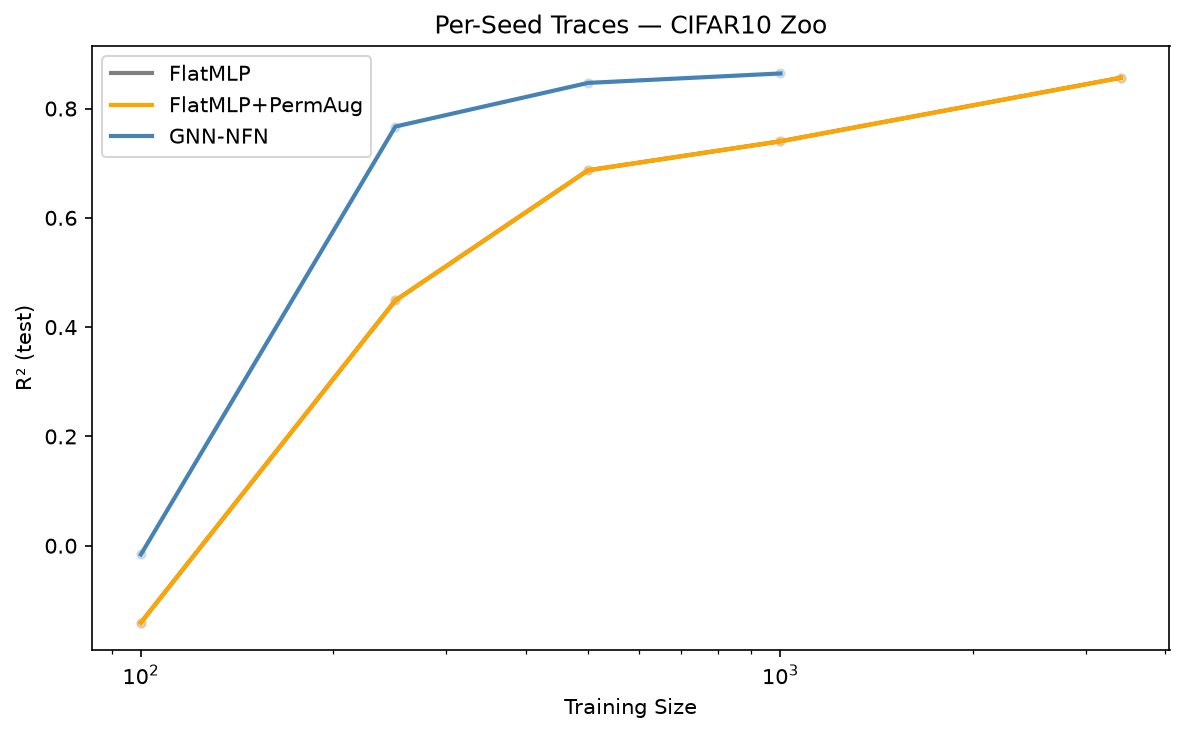
\includegraphics[width=\columnwidth]{figures/seed_traces_cifar10.png}
\caption{Seed traces CIFAR-10}
\label{fig:seed_traces_cifar10}
\end{figure}

Variance is highest at N=100, motivating multi-seed replication as the primary follow-up. GNN-NFN's variance at N=100 is visually consistent with the below-chance $R^2$ observation being a robust feature of this training scale rather than an artifact of a single unlucky seed, though confirmation requires 10-seed replication.

\subsubsection{B. Hypothesis Validation Summary}

\begin{table}[htbp]
\centering
\resizebox{\columnwidth}{!}{%
\begin{tabular}{llll}
\toprule
Hypothesis & Description & Gate type & Result \\
\midrule
H-E1 & Existence: GNN-NFN vs. flat-MLP sample efficiency on shared splits & MUST\_WORK & PASS WITH CAVEATS \\
H-M1 & Mechanism: Permutation equivariance structural verification & MUST\_WORK & PASS \\
H-M2 & Mechanism: Learning curve analysis, efficiency ratio computation & SHOULD\_WORK & PASS \\
H-M3 & Mechanism: PermAug as partial equivariance proxy & SHOULD\_WORK & PARTIAL / LIMITATION\_RECORDED \\
\bottomrule
\end{tabular}
}
\end{table}

Overall pass rate: 3 of 4 hypotheses fully or substantially validated; 1 partially validated with scientifically novel finding.

\subsubsection{C. PermAug Mechanism Verification}

The corrected PermAug implementation in H-M3 was verified prior to training:

\begin{itemize}
\item aug\_diff = 4.118 > $1\times 10^{-6}$ (augmented samples differ from originals)
\item Dataset sizes confirmed: N=100 $\rightarrow$ 1,100; N=250 $\rightarrow$ 2,750; N=500 $\rightarrow$ 5,500; N=1,000 $\rightarrow$ 11,000
\end{itemize}

The H-E1 PermAug condition had a bug (identical random seeds for base and augmented datasets) causing PermAug and flat-MLP results to be identical in H-E1 and H-M2. All PermAug results reported in the main paper are from the H-M3 corrected implementation.

\subsubsection{D. Scope Conditions}

\begin{table}[htbp]
\centering
\resizebox{\columnwidth}{!}{%
\begin{tabular}{lll}
\toprule
Condition & Results reported to hold & Results may not hold \\
\midrule
Training set size & $N\geq 250$ (GNN-NFN > PermAug > flat-MLP) & N=100 (PermAug may dominate GNN-NFN; single-seed) \\
Encoder architecture & GNN-NFN on CIFAR-10 CNN zoo & DWSNets on CIFAR-10 CNN zoo; transformer-weight encoders \\
Zoo type & CIFAR-10 CNN zoo (~9,000 models) & MNIST MLP zoo; large-scale HuggingFace collections \\
Zoo diversity & Low-to-moderate diversity (convergent accuracy) & High-diversity zoos (wide accuracy spread) \\
Data regime & Low-to-medium ($N\leq 1,000$; efficiency advantage large) & Full data (gap narrows to <4\% $R^{2})$ \\
Target property & Test accuracy prediction & Generalization gap; other model properties \\
\bottomrule
\end{tabular}
}
\end{table}
